\documentclass[UTF8]{article} 
\usepackage{graphicx}
\usepackage{subfigure}
\usepackage{amsmath}
\usepackage{makecell}
\usepackage[utf8]{inputenc}
\usepackage[space]{ctex} %中文包
\usepackage{listings} %放代码
\usepackage{xcolor} %代码着色宏包
\usepackage{CJK} %显示中文宏包
\usepackage{float}


\definecolor{mygreen}{rgb}{0,0.6,0}
\definecolor{mygray}{rgb}{0.5,0.5,0.5}
\definecolor{mymauve}{rgb}{0.58,0,0.82}
\lstset{
	backgroundcolor=\color{white}, 
	basicstyle = \footnotesize,       
	breakatwhitespace = false,        
	breaklines = true,                 
	captionpos = b,                    
	commentstyle = \color{mygreen}\bfseries,
	extendedchars = false,             
	frame =shadowbox, 
	framerule=0.5pt,
	keepspaces=true,
	keywordstyle=\color{blue}\bfseries, % keyword style
	language = Verilog,                     % the language of code
	otherkeywords={string}, 
	numbers=left, 
	numbersep=5pt,
	numberstyle=\tiny\color{mygray},
	rulecolor=\color{black},         
	showspaces=false,  
	showstringspaces=false, 
	showtabs=false,    
	stepnumber=1,         
	stringstyle=\color{mymauve},        % string literal style
	tabsize=4,          
	title=\lstname                      
}


\title{中国科学技术大学计算机学院\\《数字电路实验》报告}
\author{}

\date{}

\begin{document}
	\maketitle
	\begin{figure}[H]
		\centering
		
\includegraphics[width=2.5in]{xiaohui.jpg}\vspace{0.5cm}\\
		\large{
			实验题目:使用Vivado进行仿真\\
			学生姓名:王章瀚\\
			学生学号:PB18111697\\
			完成日期:2019/10/28\\
		}\vspace{2cm}
		
		\large{计算机实验教学中心制\\2019年09月\\}
		\thispagestyle{empty}
		\clearpage  % 清除当页页码
	\end{figure}


	\section{实验目的}
	熟悉 Vivado 软件的下载、安装及使用\par
	学习使用 Verilog 编写仿真文件\par
	学习使用 Verilog 进行仿真,查看并分析波形文件\par
	
	\section{实验环境}
	PC 一台\par
	Windows 或 Linux 操作系统\par
	Vivado 工具\par
	vlab.ustc.edu.cn(包含 Vivado 下载安装及使用教程)\par
	
	\section{实验过程}
	\subsection{下载并安装 Vivado 环境}
	本人利用校园网直接从赛灵思官方网站下载成功。
	
	\subsection{建立 Vivado 工程}
	需要注意:工程路径应为不含空格的纯英文路径、 “Default Part”页面选择 xc7a100tcsg324-1 型号的器件\par
	\begin{figure}[H]
		\centering
		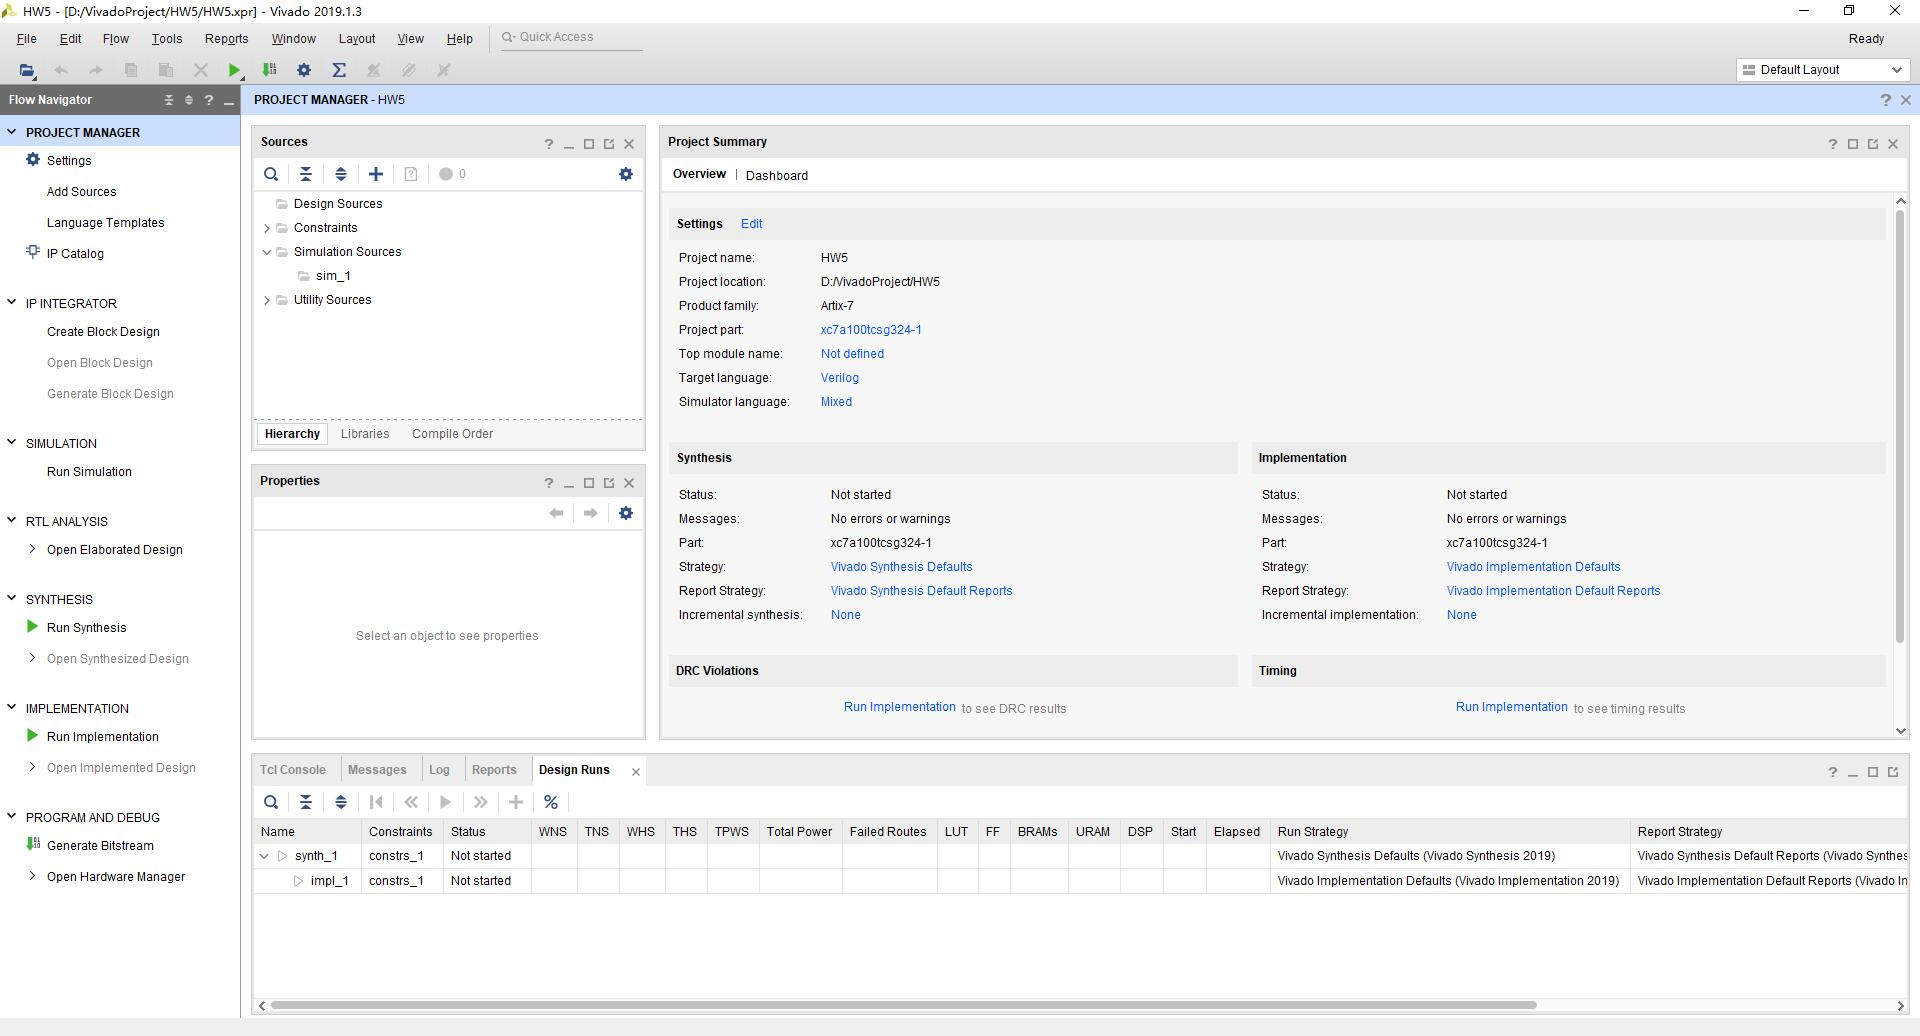
\includegraphics[width=1\linewidth]{s2.jpg}
		\label{s2}
	\end{figure}

	\subsection{添加 Verilog 设计文件}
	最终创建得到一个4bit的四选一选择器module的design文件\par
	\begin{figure}[H]
		\centering
		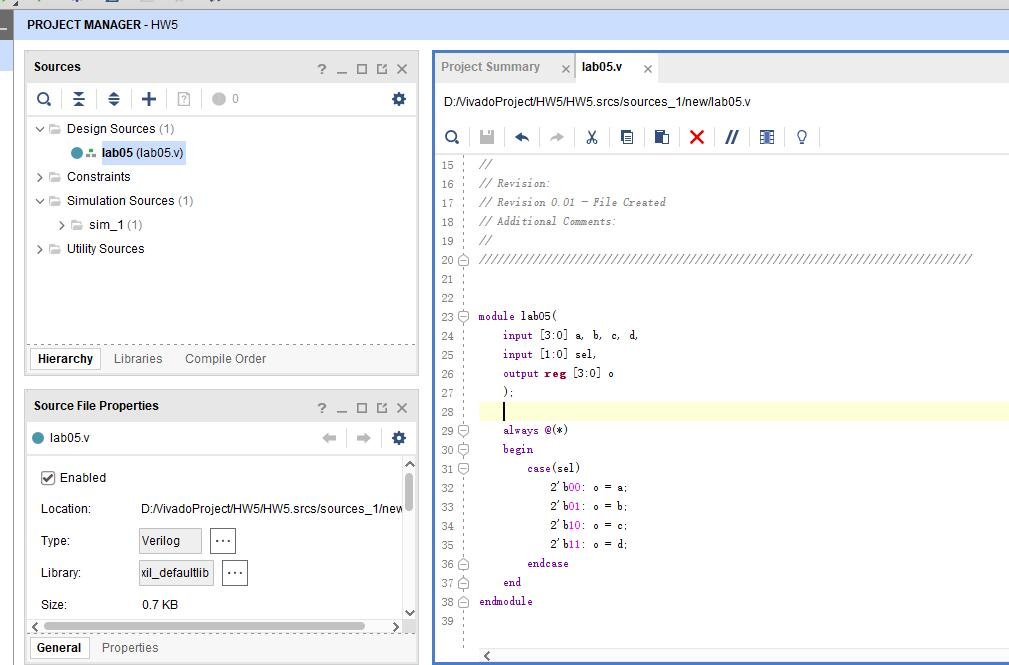
\includegraphics[width=1\linewidth]{s3.jpg}
		\label{s3}
	\end{figure}

	\subsection{添加仿真文件}
	添加结果如下:\par
	\begin{figure}[H]
		\centering
		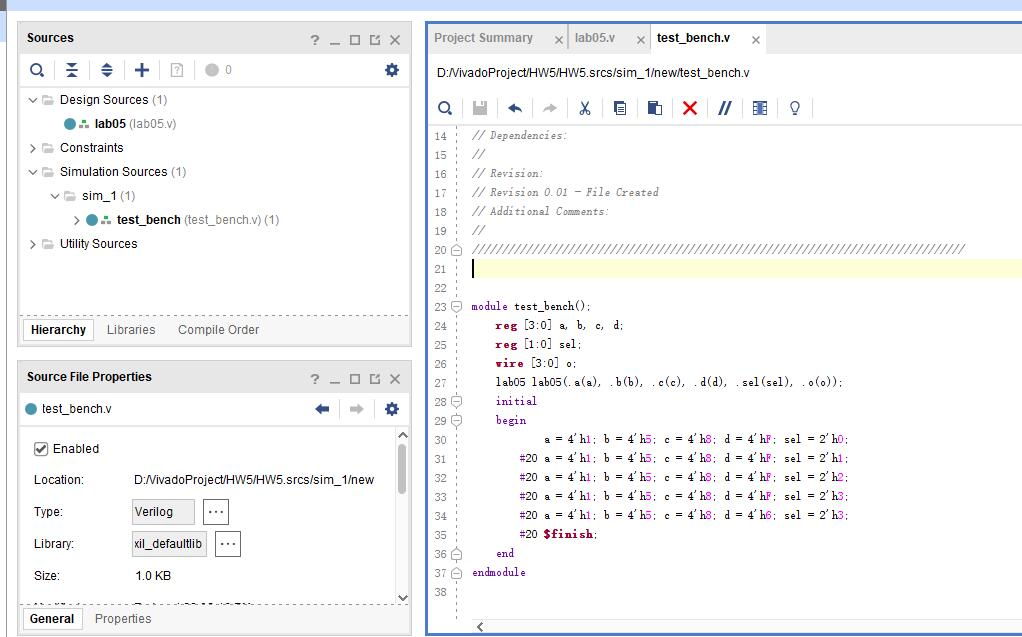
\includegraphics[width=1\linewidth]{s4.jpg}
		\label{s4}
	\end{figure}
	由上述仿真代码可以看出, Verilog 仿真文件与 Verilog 设计文件有些不同。第一,仿真文件不需要输入输出信号,所有的信号都是模块的内部信号。 第二,在仿真文件内对被测试模块进行实例化,并对被测试模块构造输入信号。第三,仿真文件只用于仿真,最终不会被综合成电路,会经常用到“initial”等 Verilog 设计文件中不会用到的关键字或语法,这些语法很多是不可综合的。\par
	
	
	\subsection{波形仿真}
	仿真结果如下:\par
	\begin{figure}[H]
		\centering
		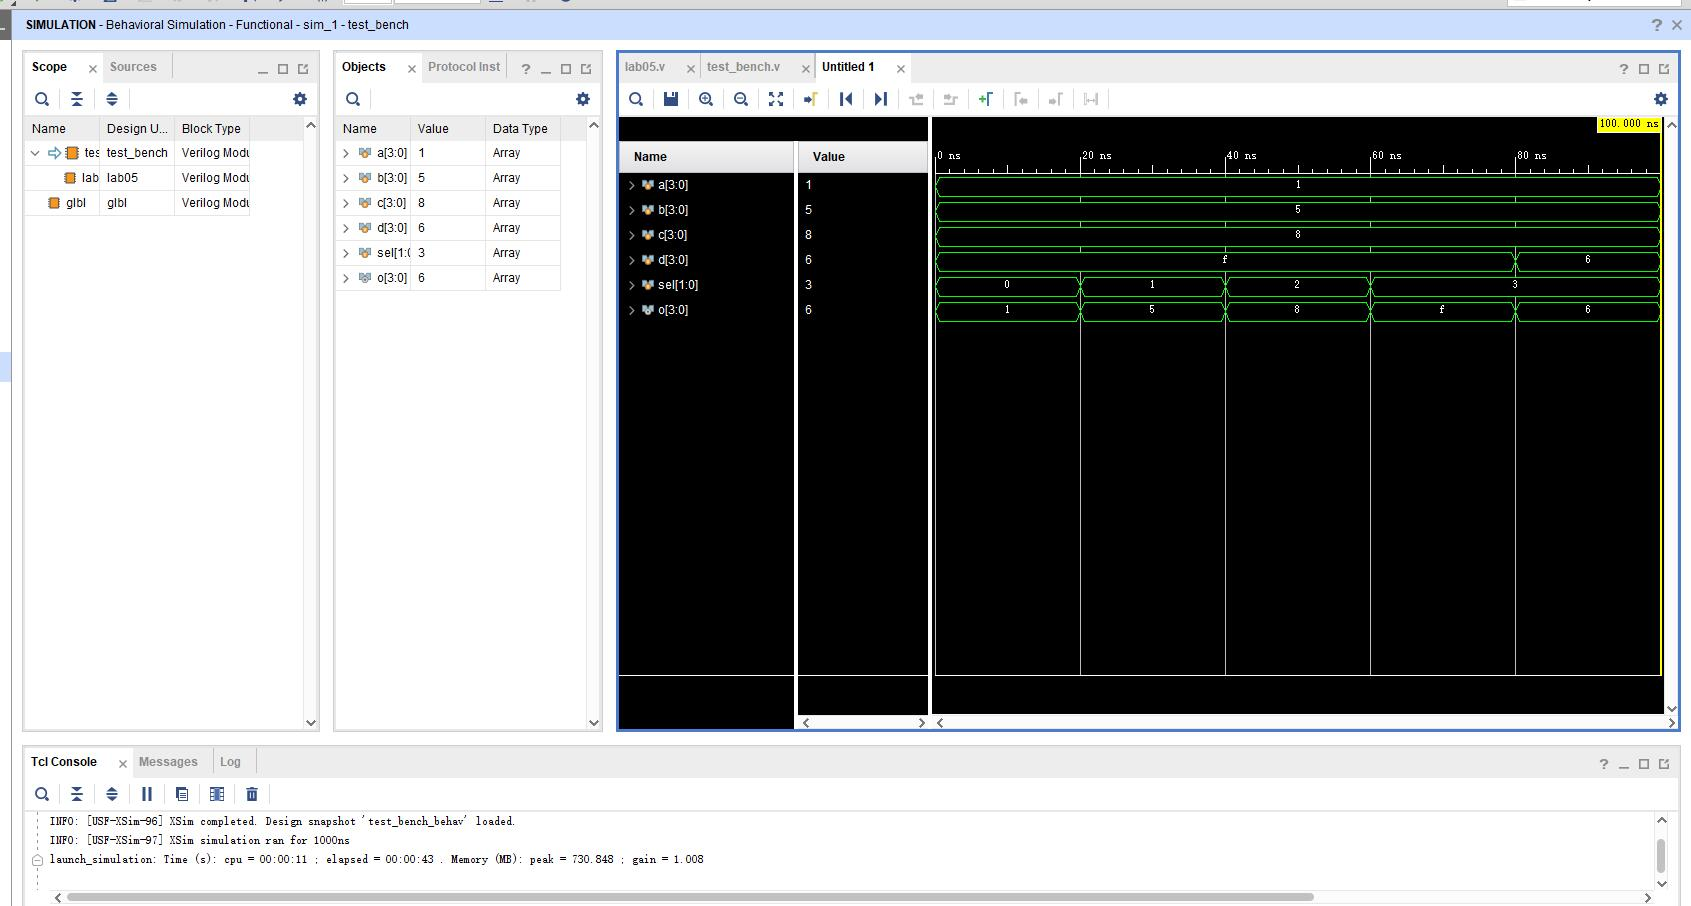
\includegraphics[width=1\linewidth]{s5.jpg}
		\label{s5}
	\end{figure}\par
	将"input [1:0] sel",改成"input sel"后,会得到如下奇怪的波形,此时容易查出错误。
	\begin{figure}[H]
		\centering
		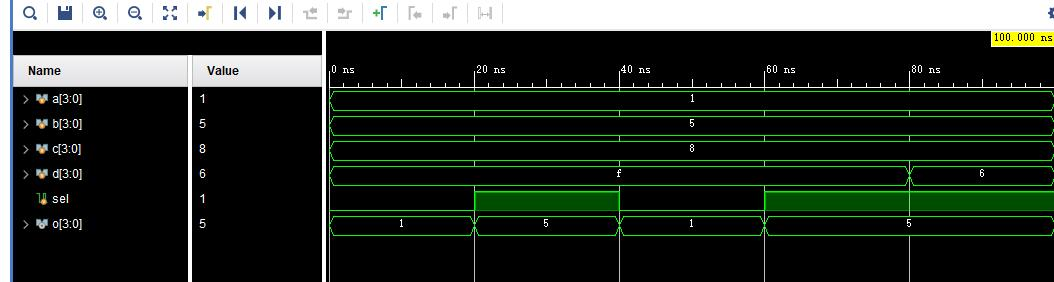
\includegraphics[width=1\linewidth]{s5_2.jpg}
		\label{s5_2}
	\end{figure}\par

	\subsection{Verilog 仿真文件常用语法}
	经学习,对原代码注释如下:
	\begin{lstlisting}[language=Verilog]
	module test_bench2();
	reg clk,rst_n,clk_a;
	reg [7:0] r1,r2,r3;
	integer i;
	initial clk = 0;
	always #5 clk = ~clk;
	
	// $stop的使用
	initial
	begin
		rst_n = 0;
		#55 rst_n = 1;
		#245 $stop;
	end
	
	// forever是循环控制的一种,表示一直执行
	initial
	begin
		clk_a = 0;
		forever #5 clk_a = ~clk_a;
	end
	
	// repeat是循环控制的一种,括号内是执行次数
	// $random%256表示在256内产生随机数
	initial
	begin
		r1 = 0;
		repeat(10)
		begin
			@(posedge clk);
			#2 r1 = $random%256;
		end
	end
	
	// for是循环控制的一种,类似于C语言的for
	initial
	begin
		for(i=0;i<20;i=i+1)
		begin
			r2 = i;#10;
		end
	end
	
	// while是循环控制的一种,类似于C语言的while
	initial
	begin
		r3=0;
		while(r3<10)
		begin
			@(posedge clk);
			r3 = r3 +1;
		end
	end
	endmodule
	\end{lstlisting}
	仿真结果如下:\par
	\begin{figure}[H]
		\centering
		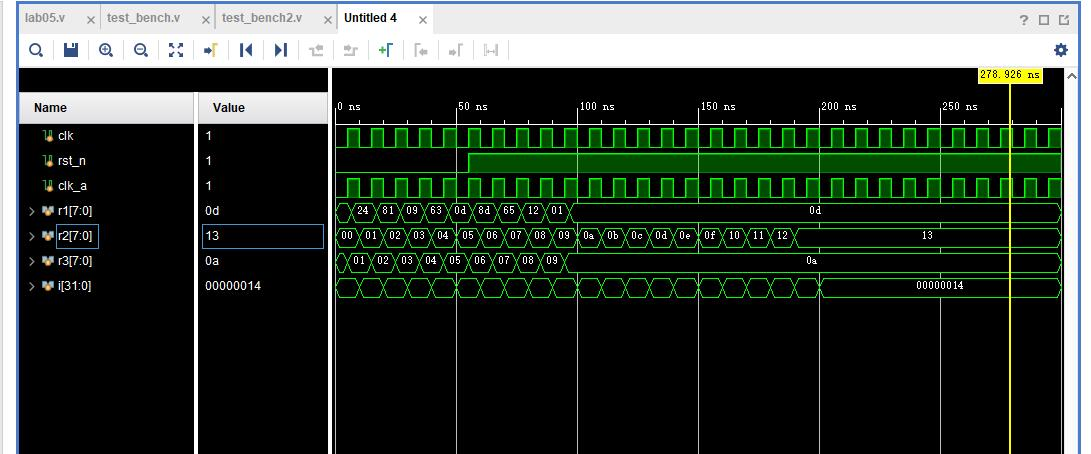
\includegraphics[width=1\linewidth]{s6.jpg}
		\label{s6}
	\end{figure}\par
	其中有些要点:\par
	\textbf{initial:}该关键字与 always 同为过程语句关键字,但与 always不同的是, initial 语句只执行一次。\par
	\textbf{时序控制:}一般用在 always、 initial 关键字后面,或者过程语句内部,常用的时序控制语句有时延控制、 电平敏感事件控制和边沿触发事件控制三种。\par
	\textbf{循环控制:} 在过程语句中可以通过循环语句实现循环控制,主要包
	括 forever、 repeat、 while、 for 四种。\par
	\textbf{系统函数:} 在 Verilog 仿真文件中支持调用一些系统函数,以提高
	仿真效率, 调用格式为:\$函数名。\par
	
	\section{实验练习}
	\subsection{题目1}
	代码如下:\par
	\begin{lstlisting}
	module e1_sim();
	reg a, b;
	
	initial
	begin
		a = 1;
		#200;
		a = 0;
	end
	
	initial
	begin
		b = 0;
		#100;
		b = 1;
		#175;
		b = 0;
		#75;
		b = 1;
	end
	endmodule
	\end{lstlisting}
	仿真结果如下:\par
	\begin{figure}[H]
		\centering
		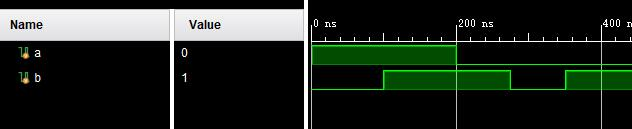
\includegraphics[width=1\linewidth]{e1.jpg}
		\label{e1}
	\end{figure}\par

	
	\subsection{题目2}
	代码如下:\par
	\begin{lstlisting}
	module e2_sim();
	reg CLK, RST_N, D;
	
	initial
	begin
		CLK = 0;
		forever #5 CLK = ~CLK;
	end
	
	initial
	begin
		RST_N = 0;
		#27;
		RST_N = 1;
	end
	
	initial
	begin
		D = 0;
		#13;
		D = 1;
		#25;
		D = 0;
	end
	endmodule
	\end{lstlisting}
	仿真结果如下:\par
	\begin{figure}[H]
		\centering
		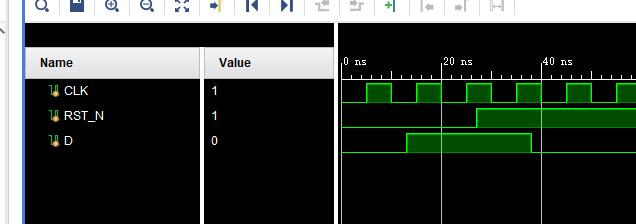
\includegraphics[width=1\linewidth]{e2.jpg}
		\label{e2}
	\end{figure}\par

	
	\subsection{题目3}
	仿真文件代码修改如下:\par
	\begin{lstlisting}
	module e2_sim();
	reg CLK, RST_N, D;
	
	// 修改处
	d_ff_r d_ff_r_init(CLK, RST_N, D);
	
	initial
	begin
	CLK = 0;
	forever #5 CLK = ~CLK;
	end
	
	initial
	begin
	RST_N = 0;
	#27;
	RST_N = 1;
	end
	
	initial
	begin
	D = 0;
	#13;
	D = 1;
	#25;
	D = 0;
	end
	endmodule
	\end{lstlisting}
	仿真结果如下:\par
	\begin{figure}[H]
	\centering
	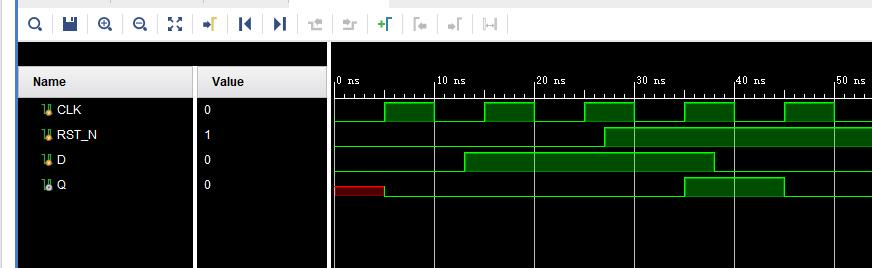
\includegraphics[width=1\linewidth]{e3.jpg}
	\label{e3}
	\end{figure}\par
	
	
	\subsection{题目3}
	仿真文件代码修改如下:\par
	\begin{lstlisting}[name=3-8译码器]
	module decoder_3_8(
		input [2:0] in,
		output reg [7:0] out
		);
	
	always @(*)
	begin
		case(in)
			3'b000: out = 8'b0000_0001;
			3'b001: out = 8'b0000_0010;
			3'b010: out = 8'b0000_0100;
			3'b011: out = 8'b0000_1000;
			3'b100: out = 8'b0001_0000;
			3'b101: out = 8'b0010_0000;
			3'b110: out = 8'b0100_0000;
			3'b111: out = 8'b1000_0000;
			default: out = 8'b0000_0000;
		endcase
	end
	
	endmodule
	\end{lstlisting}
	
	\begin{lstlisting}[name=对应仿真文件]
	module decoder_3_8_sim();
	reg [2:0] in;
	wire [7:0] out;
	
	decoder_3_8 decoder_3_8_inst(in, out);
	
	initial
	begin
		in = 3'b000;
		forever #5 in = in + 1;
	end
	
	endmodule
	\end{lstlisting}
	仿真结果如下:\par
	\begin{figure}[H]
		\centering
		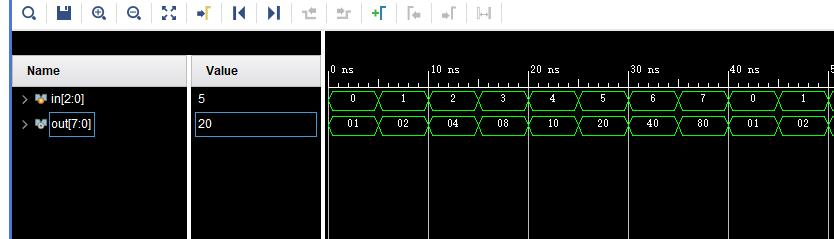
\includegraphics[width=1\linewidth]{e4.jpg}
		\label{e4}
	\end{figure}\par
	
	
	
	
	\section{总结与思考}	
	\subsection{本次实验的收获}
	在本次实验中,收获较大,学会了使用Vivado的仿真。\par
	
	\subsection{评价本次实验的难易程度}
	本次实验内容难度适中。\par
	
	\subsection{评价本次实验的任务量}
	本次实验任务量合理。\par
	
	\subsection{为本次实验提供改进建议}
	建议详述语法方面的问题。
	
\end{document}
